\chapter{Analysis of Twitter's Social Structure}

In the previous chapter, a series of studies were conducted into Twitter with respect to message propagation through retweeting. In particular, research was done to provide an understanding of the patterns produced through retweets and how their properties relate to the Twitter users that the Tweets `pass through'.

Of particular interest, however, is the social graph underlying Twitter, which describes how the users are interconnected and which dictates the information flow between them. It has been discussed that users with a higher follower count are more likely to have their Tweets retweeted, due to there being more users available to \textit{see} the Tweet, and that some users can have their Tweets forwarded through many hops indeed, so that information may be passed between different communities of users.

In addition to the effects of user influence,  several other factors also govern an individual retweet decision of a given user for a particular Tweet. These include properties of the Tweet, such as whether, or not, the Tweet contains a URL, whether it mentions a particular user, whether the user even has an opportunity to \textit{view} the Tweet, and so on.\\
These factors account for the individual user's retweet decision and the almagamation of every user's retweet decision on the Tweet describes the Tweet's overall retweetability, which essentially determines how far the Tweet can propagate.

However, it is believed that the topology of the network, below the level of user influence and other factors, can play an important role in facilitating (or inhibiting) Tweet propagation by opening and closing available retweet pathways between users and groups of users.\\
Whilst retweet decisions based on Tweet features alone, such as the actual content of the Tweet or the contents of a document a URL in the Tweet points to, may imply a level of interest in the Tweet, the influence of users has a very large impact on how many retweets a certain Tweet receives. Thus, abstracting the concepts away from user influence may help in discovering methods for deducing which information is actually interesting.

Twitter's social structure has earlier been described as being built from users creating edges between themselves through the act of \textit{following}. A followship defines the direction of travel of information from the follower to the friend, and this illustrates how users with many followers immediately have their Tweets made available to many more users before any retweeting even takes place.\\
As more edges are constructed between users the global initial spread of Tweets is increased, and, when the addition of retweets is considered, this has an larger effect. Although other intervening factors have been mentioned earlier, such as the notion of a user's network awareness and of user influence, the organisation of users on the graph and the differences in observed propagation pattern is an interesting route for research towards uncovering the properties surrounding interestingness.

In this chapter, various social network structures are constructed in order to simulate retweet behaviour between users on Twitter. The behaviours are studied with the aim to research the propagation patterns observed in different network structure types. Non-realistic and realistic graphs are built in order to highlight the low-level propagation characteristics in these networks and the similarities between more realistic simulated networks and Twitter's own social graph.\\
This research is then used to generate a methodology for estimating Tweet interestingness based on an \textit{expected} Tweet popularity, as is discussed further later in the chapter.


\section{Observing Differences in Propagation Patterns Between Different Network Structures}
In the previous chapters it has been realised that certain Tweets with particular properties may imply a certain quality that affects a user's retweet decision on the Tweet. However, in addition to Tweet quality, of interest also is the potential presence of a graph `quality', in that particular network structures may possess benefits for propagation, or at least have an effect on how Tweets are spread.

In this section, to help in addressing this research area, simulations are carried out in three different network topologies - a path (or `linear') network, a random network, and a scale-free network. In the experiments, individual user \textit{decisions} are used as the bases for demonstrating retweet behaviour.  

The simulation algorithm and ideas behind the model used for generating the simulated users' retweet decisions are adapted from the work carried out in \cite{zhu11} and \cite{peng11}, which introduces methodologies for illustrating Tweet spread through a given network of users, and the simulations can be used to produce a retweet group for a given Tweet.\\
From the analyses of the simulation experiments, of interest is whether, and how, changing the network structure does affect retweet propagation patterns, and whether a simulation can mimic Twitter's own behaviour in terms of retweet spread.

Measuring retweet behaviour is carried out through studying the distribution of retweet group sizes that result from running the experiments, as is described in later sections.


\subsection{Overview of the Simulation Algorithm}
The algorithm covers the simulation of Tweet propagation through a given set of connected users by emulating retweet decisions of each user who receives the Tweet. The retweet decision is made using a prediction based on a logistic regression classifier, as is described below.

\cite{zhu11} developed a simulation algorithm which was found to be capable of accurately predicting retweet decisions using a logistic regression. These methods were modified and adapted to fit the purposes of the simulation algorithm used in this section.\\
In essence, the simulation initially requires a graph of connected users, $U$, and a Tweet, $t$, which will be introduced to the graph and retweeted between the users. It begins by initialising a set of users, $S$, to contain the followers of a particular $u_s \in U$, which represents the user $\aut{t}{O}$. As such, users in $S$ form the set of users to have $t$ or a retweet of $t$ currently on their home timelines and available to retweet. In this case, $t$ is used to denote both the original Tweet and any copies of it made through retweeting.\\
The procedure then iterates over timesteps, at each stage checking the retweet probability of each $u \in S$. If $u$'s retweet probability is suffuciently great for $t$, then $u$ retweets $t$ by being removed from $S$ and then added to $\rt{t}$, which represents the set of users who have retweeted $t$. The followers of $u$ are then added to $S$, since these users now also hold $t$ and have the chance to make the retweet decision.\\
A threshold value, $TH$, is used to emulate the notion of the Tweet `decay' experienced when one users a Twitter client or the web interface. The reasoning behind this is that as time goes by, more and more Tweets arrive onto the recipients' home timelines. This pushes the previous Tweets further down, whether they are interesting or not. Tweets may be ignored and not retweeted if the user has not viewed their home timeline for a while or if the user decides the Tweet is not of a sufficient quality to retweet it. If a Tweet is pushed down to the extent that is out of view, or out of the current page, then the chance of that user retweeting that Tweet is reduced. Thus, if a user is in $S$ for more timestep iterations than specified by $TH$, then the user is removed from $S$, meaning that it can no longer have the chance to retweet the Tweet.\\
Users who have retweeted $t$, or are unable to do so (either by having previously retweeted it or by exceeding $TH$) are prohibited from being (re-)added to $S$.

The algorithm terminates either when the timesteps thus far iterated exceed the maximum allowed, $T$, or when $S$ becomes empty. This results in the retweet group, $\rg{t}$, which comprises the final set, $\rt{t}$, along with the initial $u_s$. As in the previous chapter, $\rc{t} = |\rt{t}|$.

Therfore, the additional necessary components to run the simulation are the facilities for building a user graph, a constructed Tweet, and functionality for generating a retweet probability for each user who receives the Tweet.

\newfloat{algorithm}{H}{lop}
\begin{algorithm}
\caption{Simulation of retweet decisions on $t$ in a given network of users, $U$}
\begin{algorithmic}[1]
\Procedure{simulate}{graph of users $U$, tweet $t$}
    \State $RT\gets$ empty set \Comment{To hold users who retweet $t$}
    \State $T\gets$ number of timesteps allowed
    \State $TH\gets$ maximum timesteps \Comment{Emulate $t$ `slipping down' timeline}
    \State $us\gets$ source User selected from $U$
    \State $S\gets$ initialise to followers of $us$
    \Statex % new line
    \ForAll{$ti$ in range $(0,T)$}
        \ForAll{$u \in S$}
            \State $P\gets$ retweet probability of $u$ on $t$ in range $(0,1)$
            \State $r\gets$ random number in range $(0,1)$
            \If{$P > r$}
                \State Remove $u$ from $S$
                \State Add $u$ to $RT$
                \State Add followers of $u$ to $S$
            \Else
                \State Increment $u.\textrm{TIME\_HELD}$
                \If{$u.\textrm{TIME\_HELD} > TH$}
                    \State Remove $u$ from $S$ \Comment{$u$ has held $t$ for too long in timeline}
                \EndIf
            \EndIf
        \EndFor
        \If{$|S| = 0$}
            \State Return $RT$ \Comment{No more users can retweet $t$}
        \EndIf
    \EndFor
    \State Return $RT$
\EndProcedure
\end{algorithmic}
%\caption{Algorithm to simulate retweet decisions in a given network of users.}
\label{algo1}
\end{algorithm}


\subsection{Generating a User's Retweet Probability} 
As prevoiusly mentioned, \cite{zhu11} used a predictive model for retweet decisions based on a logistic regression, which was demonstrated to be capable of accurately predicting a user's retweet chance on a given Tweet. The regression was trained on a set of user, tweet and context features in order to classify a likelihood on the binary decision: retweet or no retweet, such that if $P = 1$ then the retweet will definitely occur.


\subsubsection{Machine Learning}
Machine learning is the term given to the family of techniques that allow a program to make predictions for the outcome of unseen instances based on an observed and known history of occurrences. There are many types of machine learning classifiers that are suitable for different purposes, such as for predicting an expected outcome from a set of nominal categories, for predicting a value from a continuous range, or for predicting the \textit{probability} of a binary outcome.

Most machine learning techniques involve the training of a predictive model, which contains the information on known outcomes for a set of features. The model is then used to estimate an unknown outcome, usually with a probability on the \textit{confidence} of the classification, for new sets of instances.

For example, consider three attribute variables, $A$, $B$, and $C$, each of which can be equal to one of two nominal values; \textsc{True} or \textsc{False}. A particular machine learning algorithm trains a model based on its knowledge that;
\begin{itemize}
    \item $A\gets$ \textsc{True}, $B\gets$ \textsc{False} $\Longrightarrow$ $C\gets$ \textsc{True}
    \item $A\gets$ \textsc{False}, $B\gets$ \textsc{False} $\Longrightarrow$ $C\gets$ \textsc{False}
\end{itemize}
Although training of predictive models nearly always involves using more than two instances, the history of these example instances indicate that $C$ is more strongly associated with $A$ than with $B$. As more instances are added showing similar patterns, then the association becomes stronger, to the extent that the classifier will predict $C\gets$ \textsc{True} in instances where $A\gets$ \textsc{True} (and vice versa) with higher confidence.

In this case, $A$, $B$, and $C$ are known as the `features', and a set of such features form the `instance'. Once a trained model has been constructed, the machine learning algorithm will only be able to make predictions using instance features it has knowledge of. For example, if the example classifier was now given an instance containing a feature $D$, then it will not `know' how changes in $D$ will affect $C$'s outcome.

If there is not a strong correlation between the features in a dataset, then the confidence of the classification of a particular feature will be weaker. Although this example has focussed on boolean (nominal) data types, many machine learning classifiers are able to work with features that are higher dimensional nominal values, contunuous reals, and so on, and will apply weights to the different features based on their level of influence over other features in the instance.


\subsubsection{The Logistic Regression}
Logistic regression analysis can be used as a machine learning classifier for working with binary outcomes based on a set of predictor variables (or features) \cite{hosmer13}, which makes it an appropriate approach for predicting a binary retweet decision. Logistic regressions have been frequently used in retweet analysis \cite{castillo11} \cite{zhu11} \cite{peng11} \cite{naveed11} \cite{hong11}, as discussed in the Background chapter.

An implementation of the logistic regression algorithm was written in the Python programming language, which formed the basis of calculating the value for the retweet probability, $P$, based on a set of feautures of the Tweet and author user.


\subsection{Summary of Training Features}
\cite{zhu11} used the approach in order to accurately model retweet decisions in Twitter. A set of around 50 different features were used to train the logistic regression, with the retweet outcome (\textsc{True} or \textsc{False}) being the predicted classification in each case. These features included Tweet-related features (such as content analysis, inclusion of URLs, etc.), and network and user features (followships, mentions, etc.).

Since the network structures themselves, and the propagation \textit{patterns}, are what are of interest in this section, the simulation is significantly simplified by using far fewer features, yet ones which are features that have been shown to have a strong influence on the retweet decision. As long as a consistent set of feature groups and values are used, the properties of the retweet groups observed should demonstrate the varying behaviours across the different user structures.

As such, each instance comprised the following four features associated with each Tweet, $t$, and where $u$ is the user currently making the retweet decision, \textsc{retweet};

\begin{table}[h]\footnotesize
\begin{center}
\begin{tabular}{ l | c | l }
	Feature & Data type & Description\\
	\hline
	\hline 
	\textsc{follows}    & \{\textsc{True, False}\} & \textsc{True} if $u \in \fos{\aut{t}{O}}$\\
    \textsc{followed}   & \{\textsc{True, False}\} & \textsc{True} if $u \in \frs{\aut{t}{O}}$\\
    \textsc{mentioned}  & \{\textsc{True, False}\} & \textsc{True} if $u$ is mentioned in $t$'s content\\
    \textsc{url}        & \{\textsc{True, False}\} & \textsc{True} if \texttt{http://} or \texttt{https://} in $t$'s content\\
    \hline 
    \textsc{retweet}    & \{\textsc{True, False}\} & \textsc{True} if $u \in \rt{t}$\\ 
    \hline
\end{tabular}
\end{center}
\caption{Training features for the logistic regression.}
\label{table:logisticregressionfeatures}
\end{table}

The \textsc{url} feature has, in the literature, often been found as a large impacting feature on retweets in Twitter, especially in \cite{alonso10}, who use it as their basis for determining .nd identifying interesting Tweets.


\subsection{Training the Model}
In order to train the logistic regression model, data was required from Twitter so that the sets of feature instances could be built. 

Data collection for these experiments again utilised Twitter's REST API, which was queried between March and June 2012 to collect a set of around 12,000 Tweets and retweets. Since these dates were before the mandatory switch-over to v1.1 of the REST API, the public timeline could again be used to collect the data without the necessity of crawling through the social graph.\\
In this case, it was particularly necessary that non-retweets were also collected in order to provide the negative case when training the regression model and to ensure that there were instances where the \textsc{retweet} feature could be \textsc{False}.

In cases where the collected Tweet was a retweet, further calls were made to the API to determine the relationships between the retweet's author and the original Tweet's author in order to satisfy the required \textsc{follows} and \textsc{followed} features.
Where the collected Tweet was not an instance of retweet, there is no original author to examine the relationships between. In these cases, further Tweets were retrieved for the user in order to find their retweet rate in terms of the ratio of retweets to Tweets on their user timeline and an analysis of the relationship between these and the original authors. This was used in conjunction with the user's follower and friend count to determine a probability of the `faux' followships. As mentioned, the accuracy of the retweet counts obtained through the simulations is not particularly important; of interest is the propagation patterns observed over the graph structures.

After storage, the regression model was trained using features extracted from the raw data, which the simulation algorithm could then use to generate the required retweet probability, $P$.


\subsection{Running the Simulations}
Once the model had been trained, the simulations could be run. In each simulation experiment, a network of users was generated, as described in the next section, and a Tweet object was created.\\
This Tweet object contained information on whether or not it contained a URL and if it mentioned one of the users in the generated network. 

Various parameters - such as $TH$, the size of the user network, $U$ to be generated, $t$'s Tweet features, and any weightings on the decision probability prediction generator - could be altered to affect the strength or correlation of the patterns produced by the different network structure types in the simulations.


\subsection{Network Analyses}
In this section, three network structures are assessed in terms of the differences in the patterns of propagation each expresses. Each generated graph is \textit{directed} in order to illustrate the followships between the user nodes, and to support the use of the \textsc{follows} and \textsc{followed} features required in the decision probability calculation.

In each case, the same set of generated Tweets were used, but different structures required the various parameters to be set slightly differently and, as such, each network structure will present with different proportionate retweet group size distributions when highlighting the different patterns.


\subsubsection{Path Network}
The first assessed structure was to illustrate the pattern on a non-realistic social network structure; a path network.

Path networks are one of the simplest type of graph, and a linear directional path network consists of the graph of users, $U$, of size $n$, in which each user $U_i \forall 0 \leq i < n$ is followed by user $U_{i+1}$. As a result, each $u \in U$ has precisely one follower and one friend, except the users $U_n$ and $U_1$ respectively.\\
$n$ is the only parameter necessary in the construction of this user graph.

\begin{figure}[h]
\centering
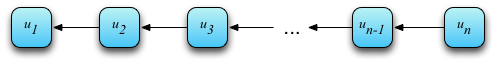
\includegraphics[scale=0.8]{4.Chapter2/Media/path_network.png} 
\caption{Example of a path network.}
\label{fig:path_network}
\end{figure}

In this graph, the size of the retweet group is, by definition, equal to the depth of penetration, as there is only one path (or retweet chain) available for propagation to occur down. As such, in each case, the retweet tree representing a resultant retweet group formed in this type of network will have the same structure as the graph itself, yet with a size dependent on the collective retweet decisions of the users.

Since each internal user has only one follower, the likelihood of a retweet decision being positive at each timestep is somewhat progressively reduced, and thus the retweet count is much more likely to tail off sooner than in graphs with more propagation avenues. This is also due to the fact that each retweet can only reach an audience of size 1 at each time step, and thus the `survival' of the Tweet cannot rely on a summation of many users' retweet decisions. 

\begin{figure}[h]
\centering
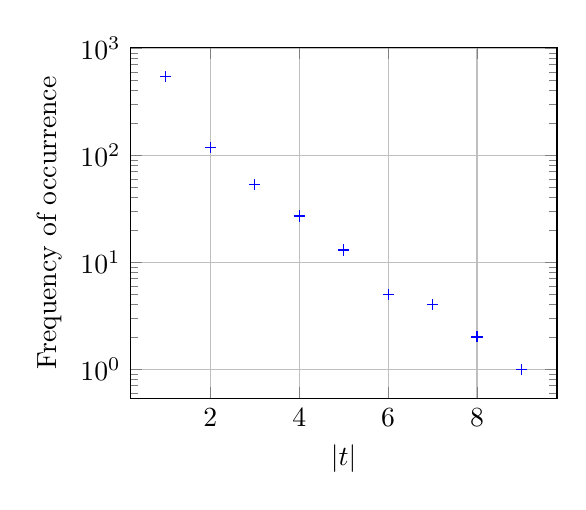
\begin{tikzpicture}
 \begin{semilogyaxis}[
        xlabel=$|\rg{t}|$,
        ylabel=Frequency of occurrence,
        width=7cm,
        grid = major]
    \addplot[only marks,mark=+,blue] plot coordinates {
        (1,540)  (2,118)  (3,53) (4,27) (5,13) (6,5) (7,4) (8,2) (9,1) (10,0)
    };
\end{semilogyaxis}
\end{tikzpicture}
\caption{Frequency distribution of retweet group sizes in path network simulations}
\label{fig:linear}
\end{figure}

The likelihood of a particular user achieving the opportunity to receive the Tweet, in order to then retweet it, becomes the product of the probability function the further it travels through the graph, in which user $U_i$ requires each user from $ U_1$ to $U_{i-1}$ to first make a positive retweet decision. For example, if each user has probability $p$ of retweeting the Tweet, then each user's chance of retweeting the Tweet is $\frac{1}{p^i}$, where $i$ is the position of the user in the graph.

Therefore, as might be expected, the frequency distribution of retweet group sizes shows a half-life type behaviour demonstrating the logarithmic pattern with many small retweet groups followed by a series of exponentially smaller groups.\\
This user structure illustrates well how some users that might find the Tweet interesting, and who may then decide to retweet it, do not even get the chance to view it in order to \textit{make} that decision. Although this is accentuated in this structure, the same principle applies to any non-complete social graph, and demonstrates how the way users are connected can have a large impact on the retweetability of a particular Tweet.


\subsubsection{Random Network}

\begin{figure}[h]
\centering
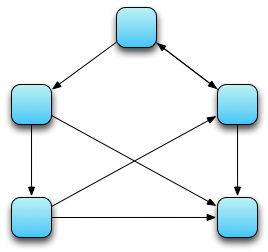
\includegraphics[scale=0.8]{4.Chapter2/Media/random_network.png} 
\caption{Example of a random network where $n = 5$ and $p \sim 0.5$.}
\label{fig:path_network}
\end{figure}


The random network was the next user structure to be analysed. Although it is certainly more similar to a real-life social graph than a path network, it is much more basic and uniform and does not consider user communities and clusters or different levels of influence in users in terms of differences in follower and friend counts.

A random social network is defined as the case in which the graph of user nodes, $U$, and where $n = |U|$, consists of each user, $u$, having probability $p$ of following each other $u_i \in U \forall 0 \leq i \leq n$ and where $u_i \neq u$. Thus, as $p$ is increased, then the likelihood of $u$ following a $u_i$ increases, causing the overall network edge density to increase. In general, therefore, the average number of followers and friends of a user is proportional to $p.n$.\\
The only parameters needed for constructing such a graph are $n$ and $p$.

\begin{figure}[h]
\centering
\begin{tikzpicture}
 \begin{semilogyaxis}[
        xlabel=$|\rg{t}|$,
        ylabel=Frequency of occurrence,
        width=7cm,
        grid = major]
    \addplot[only marks,mark=+,blue]
       file {4.Chapter2/data/random.dat};    
\end{semilogyaxis}
\end{tikzpicture}
\caption{Frequency distribution of retweet group sizes in random network simulations}
\label{fig:random}
\end{figure}

The frequency distribution demonstrates a very large proportion of mid-range values for $|\rg{t}|$, indicating that Tweets tend to have a consistent spread amongst the network, as might be expected. There are few smaller groups since there are no users that have disproportionately smaller spheres of influence, and each user has many incoming edges and a similar number of outgoing edges. As such, there are more mid-range retweet group sizes than smaller ones.\\
However, as in any distribution so far examined, the distribution of retweet group sizes must eventually tail off due to the natural eventual reduction in positive retweet decisions being successively made as retweet chains increase in length.


\subsubsection{Scale-Free Network}
The final network structure examined in this section is the scale-free network. Also known as `small world', scale-free graphs are generally known to be representative of the general structure of `real-life' and online social networks \cite{mislove07} and, indeed, they are also used to describe the interconnections of real-world properties, such as friendship groups and food webs \cite{guido07} \cite{hein06}.\\
Essentially, scale-free networks dictate that there are a small number of nodes with a high degree and many nodes with a low degree, and are usually generated through some form of preferential attachment algorithm. Thus, this type of network has support for the consideration of user communities and influential users in terms of those demonstrating a disproportionately large follower count. The other user structures studied do not have the scope for emulating this property of inconsistent interconnection between the user nodes.

Scale-free networks are constructed such that the distribution of the degree of the graph's nodes follow a power-law in that the distribution of the number of vertex edges across the graph is logarithmic.\\
For these analyses, NetworkX\footnote{http://networkx.lanl.gov}, a Python graph and networking package, was used to generate directed scale-free graphs of users, which essentially accepts a network size, $n$, and edge density $d$ as the graph construction parameters. 

\begin{figure}[h]
\centering
\begin{tikzpicture}
 \begin{loglogaxis}[
        xlabel=$|\rg{t}|$,
        ylabel=Frequency of occurrence,
        grid = major,
         legend style={at={(0.5,-0.27)},anchor=north,legend cell align=left},
        legend entries={Twitter data, Generated scale-free data}]
    \addplot[only marks,mark=*,red]
       file {4.Chapter2/data/comparison-real.dat};
    \addplot[only marks,mark=*,blue]
       file {4.Chapter2/data/comparison-scale-free.dat};
\end{loglogaxis}
\end{tikzpicture}
\caption{Comparison of retweet group size distributions from scale-free graph simulations and data from Twitter's own social graph.}
\label{fig:real-scalefree}
\end{figure}

From simulations of the algorithm through these scale-free networks, a logarithmic trend is observed similar to that demonstrated from the `real' Twitter data analysed in the previous chapter and published in \cite{webberley11}, and the similarities in the distribution pattern is illustrated by Figure \ref{fig:real-scalefree}.


\subsection{General Comparison of Propagation Characteristics across Different Graph Structures}
In this section, three different network structures have been compared, and whilst the path network is very unrealistic as a representation of a social network, the differences in propagation behaviour presented by each do show how the interconnection of users on the graph can have a large effect on the spread of a Tweet. A small set of features to govern retweet features were used in order to accentuate the difference made by the user structures themseleves.

This has demonstrated that, in addition to the processes behind a user's individual retweet decision, the eventual spread of a Tweet also depends somewhat on how the original author's local network is arranged. Thus, the retweet decision of each involved user along with the available information pathways provided by the underlying social structure both contribute to the overall retweetability of a Tweet. 

If there are many edges in the network, such as in the case of the random network, then there are many more routes for peopagation to occur down to and from each user, due to the relatively large in- and out-degree of each user node on the graph. This increases the number of users who end up receiving the Tweet and then have the chance to make a retweet decision. This resulted in there being a larger distribution of larger retweet group sizes than smaller ones, before naturally diminishing again. Despite this high throughput of retweets, which provides a high level of information \textit{recall} for the users, the random graph structure is likely to demonstrate a low \textit{precision} in terms of the interestingness of the received Tweets.\\
This is due to the large number of users having the opportunity to retweet the Tweet, increasing the chance that the `noisy' information will be filtered through.

The path network demonstrated very poor propagation, and required that its simulation parameters were altered to facilitate retweet behaviour significantly more than in the other graph structures in order to produce any observable pattern. The results showed that propagation down a single allowed chain cannot be an effective way to spread Tweets, as it required each user in the chain to retweet it so that the successive users can have a chance to view it.

Whilst the scale-free network does not have the same general propagation throughput as the random network, it does demonstrate retweet patterns similar to those observed in data from Twitter's own social graph. This complements the findings of \cite{mislove07} and \cite{hein06} in terms of online social networks emulating real-life social networks having scale-free properties.\\
This type of structure supports areas of the graph with denser communities, as is shown to exist by \cite{java07}, and have the potential for facilitating very large numbers of retweets if influential users are involved, but illustrate how Tweets `travelling' through less dense areas (and less-influential users) will not be as demonstrably popular.



\section{Using the Social Graph as a Method for Inferring Interestingness}
The graph analyses in the previous section have demonstrated a method for generating a $\rg{t}$ for a given Tweet, $t$. Since $\rc{t} = |\rg{t}| - 1$, then the same simulation algorithm can be used to estimate a retweet count for a given Tweet. Although it has been discussed that although an individual user's retweet decision does generally imply that user's interest in the Tweet, the overall retweet count of a Tweet is only really capable of denoting that Tweet's popularity. However, this value could be used in tandem with the predicted expected retweet count of a Tweet in order to determine if the Tweet is, in fact, interesting.

This notion is based on the idea that if a Tweet is more popular than expected, then there is something about that Tweet that makes it more \textit{interesting} than similar Tweets that are less popular, such as some breaking news or a link to a controversial article.\\
For example, consider the case of two Tweets, written by the same author, and both containing the same instances of feature values, such as the inclusion of a URL or a mention. If one of these Tweets achieves significantly more retweets than the other, then there must be some non-trivial feature of the more popular Tweet that makes it stand out to the audience, and thus allows it to be perceived as more \textit{interesting}. This is because the features taken into account are very static, and do address any depth of the actual content of the Tweet.\\
Similarly, if most Tweets of a user achieve between one and two retweets, then the expected retweet count for this user's future Tweets is likely to be similar. If, however, the author posts a Tweet which achieves an observed total of 10 retweets, then this is more popular than what was expected. If a Tweet achieves one or zero retweets, then this is as expected or less than expected, and is therefore not interesting.

As such, a method is proposed based on the following two criteria;
\begin{itemize}
    \item observed $\rc{t} >$ expected $\rc{t} \Longrightarrow t$ is interesting
    \item observed $\rc{t} \leq$ expected $\rc{t} \Longrightarrow t$ is non-interesting
\end{itemize}

Although it was found, in the previous chapter and in other relevant literature, that pseudo-generated scale-free networks can be representative of Twitter's own social structure, a user's actual own local social network would more accurately portray the links between the users surrounding the original author of a Tweet. By constructing a network based on a user's own local network, then the method would effectively be simulating the Tweets' propagation through the edges representing the followships of the actual users in Twitter's social graph.

Thus, in the simulation algorithm, the user in question is $u_s$, and the intiial value of $S = \fos{u}$. At each timestep, each user in $S$ would have the opportunity to retweet the Tweet, and therefore, by running the simulation, an estimation on the \textit{expected} value for $|\rg{t}|$ can be obtained, where $\aut{t}{O} = u_s$.\\
In particular, the method follows these steps;
\begin{enumerate}
    \item Select a user, $u$
    \item Collect that user's local follower network 
    \item Collect a set of that user's recent Tweets
    \item Construct a network based on the users and edges of the collected network
    \item Simulate the collected Tweets through the constructed network using the simulation algorithm using $u$ as the Tweet's source author user.
\end{enumerate}

This procedure would provide an estimated retweet group size for each Tweet, which could then be compared to the actual observed retweet count of the Tweet on Twitter to help towards deducing the interestingness.


\subsection{Data Collection}
Due to the scaling properties encountered in a breadth-first traversal of Twitter's social graph, it became infeasible to collect a user's local network containing users more than two edge `hops' away from the source user under the rate limitations of Twitter's REST API.\\
As previously described, v1 of the REST API allowed 350 calls to the API each hour for each authenticated Twitter account. One call, for example, was required to obtain a list of up to 5,000 user IDs representing the followers of a particular user - the users one hop from the source user. An additional call would then be required to collect each of these user's own followers in order to provide the 2-hop representation of the local network from the source user.

For a user with a follower count of 700, a total of 701 API calls would be required to collect the user's local network within two hops - the one to retrieve the source user's immediate followers, and then one further call for each of the 700 followers. This would take over two hours of collection, and to collect the third hop would require another exponential number of API calls.\\
If each of the 700 followers of the source user has, on average, 200 followers, then this would require  a further $700 \times 200 = 140,000$ API calls, which, in total, equates to over 402 hours of data collection time. Although some follower overlap is likely to be present among the users two hops away, when one considers that this is simply the time taken to collect the local network for \textit{one} user, then it becomes clear that this must still be an impractical approach.

In the previous chapter it was found that the vast majority of retweets do actually occur \textit{within} two hops of the source user, in that retweet groups produced have a maximum path-length of less than three. In addition, as mentioned, online social networks are `closer' than real-life social networks, and was found to have a value of around four degrees of separation in Facebook. These points help to justify the decision made to classify a user's local network as those users and edges existing within two hops from the source user.

In June 2012, the Twitter REST API was used in order to conduct a random walk through Twitter's social graph. Starting by selecting an initial user, an edge expressing the followship of a random follower was chosen in order to select the next user. This continued for each of the selected users in turn and, for each user selected, the most recent 300 Tweets and surrounding information was collected along with that user's local follower network within two hops. The friend network (i.e. the outward edges from each user) was ignored, as only the directional outward flow of information from the source user was useful in this experiment.\\
If, at any stage, the currently selected user did not have any followers, the collection algorithm backtraced to the previous user and another follower was selected instead. The crawler continued until the rate limit for the current request window was met, at which time the current data state was stored, and then waited until the rate-limit was reset before continuing.

The data collection resulted in a set of 33 Twitter users, each with a full local network collected and a set of up to 300 Tweets. In total, around 10,000 Tweets were stored as a result of the crawl to be used in the simulations. It was decided that the previously trained regression model would be re-used as part of the retweet decision engine in this experiment also, and so no further training data was required to be collected. From the Tweets collected, the \textsc{url} and \textsc{mentioned} features could easily be indentified, and the two user features could be extracted under the same process as the one used in the network simulations in the previous section.

For each Tweet collected, a simulation could now be run in order to provide an expected retweet count for that particular Tweet. By comparing this value to the actual popularity expressed by the Tweet, which is returned as part of the standard Twitter API call, an indication of whether or not the Tweet is interesting could be obtained.



\subsection{Validating the Accuracy of Inference Results}
In order to test the validity of the results, it was necessary to use human asessment on each of the evaluated Tweets to check for agreement between the interestingness inferences made by the algorithm and by humans.\\
Although interestingness is a subjective notion, the validations were carried out in such a way to emphasise a \textit{global} level of interest in terms of the general separation between noisy and un-noisy Tweets.


\subsubsection{Crowdsourcing Validations}
Crowdsourcing is a technique that has grown in popularity over many domains in recent years, including  media, reviews services, sensor networks, and others. Essentially, crowdsourcing involves the use of many people (or, in some cases, devices) providing input or results on a given task.\\
Services such as Google Maps\footnote{http://maps.google.com}, TripAdvisor\footnote{http://tripadvisor.co.uk}, and Stack Overflow\footnote{http://stackoverflow.com} respectively use crowdsourcing for obtaining information (such as photos) on geographic locations, service reviews, and programming assistance. Its use means that the crowdsourcers can easily receive lots of input with very little additional work, since the load is spread amongst many people.

Crowdsourcing has also proved to be a useful asset in research as it facilitates the harvesting of many inputs, from diverse opinions and views, much more quickly than without it, and it is a useful tool for validating data.\\
Many crowdsourcing services are active on the Internet to cater for different use-cases. Kickstarter\footnote{http://kickstarter.com} exists as a platform for advertising a product idea or concept with the aim of achieving finance to go towards its production (known as `crowdfunding'), and Amazon's Mechanical Turk\footnote{http://mturk.com} enables crowdsourcers to employ people to carry out tasks.

Mechanical Turk allows crowdsourcers to create small jobs (known as `microtasks') to be completed by crowdsourcees, known as Mechanical Turk Workers (MTWs), who have an account on the website. The crowdsourcer describes the particular microtask in terms of what is expected of the MTWs and also determines the amount paid for the task. A single microtask completed by a particular MTW is known as a `judgment', and MTWs are paid for each judgment he/she completes. The crowdsourcer can define certain criteria on the microtasks, such as allowing each MTW to only complete one microtask.

Due, at this time, to Mechanical Turk's availability to only US credit card holders, Crowdflower\footnote{http://crowdflower.com} was used instead to submit the microtasks to Amazon's service in order to be completed by the workers. 


\subsubsection{Aims of the Validations}
The purpose of the use of crowdsourcing was for evaluating the effectiveness of the interestingness inferences made through the aforementioned comparison between an expected and observed popularity of a given Tweet. In particular, of concern was the similarity between those Tweets that the algorithm denoted as interesting and the Tweets that humans found interesting.

Since the accuracy of the various components of the technique could not be known until they were properly validated, it was decided that the crowdsourcing would initially be run as a pilot test in order to identify the presence of any correlations. If this was sufficiently successful, then a further and more rigorous test would take place, involving more crowdsourcees in order to produce a more rigid result.


\subsubsection{Constructing the Questions}
The microtasks presented to the MTWs each consisted of a question containing five Tweets. The Tweet data from the data collection was compiled into a set of questions in which each of the five Tweets were selected at random.\\
Each question asked the MTWs assessing the particular question to select which one of the five Tweets was the most interesting and which one was the least interesting, and each of the questions was assessed by at least three different MTWs.

Although Tweet selection was random, Tweets whose content starts with a user's ``@'' username (i.e. `@-replies') were excluded, since these Tweets typically form part of a conversation between a small number of users and are unlikely to convey any interest to those not directly involved in the conversation. The final validation set consisted of a total of around 4,500 Tweets to be assessed in the questions, and MTWs were encouraged to follow links to any websites or media included in the Tweets' contents as part of their evaluation of each Tweet.


\subsubsection{Inference Performance Validation Results}
Since at least three separate MTWs were responsible for assessing each question, only Tweets where two or more MTWs agreed on the interestingness of a Tweet were considered, and other instances were discarded. It is assumed that if at least two people agree on a piece of content being interesting, then this provides further strength to the judgment.\\
Through the retweet simulations and algorithm for each Tweet, an 86\% accuracy was achieved in terms of correctly predicting the actual retweet count - the cases where the expected retweet count is equal to the observed retweet count. In around 30\% of cases, a Tweet that was determined to be interesting through the methodologies described in this chapter was also verified as interesting by the agreeing MTWs.

This is a relatively low accuracy, and while it does mean that the method was able to correctly identify an interesting Tweet from a set of five in 30\% of cases and the random performance of selecting an interesting Tweet could not reach this accuracy, it is not a strong enough result to describe the method as being suitable in the general inference of interesting Tweets. 

As such, further investigation would be required to address the method with the aim of improving this performance.


\subsection{Improving The Interestingness Inference Performance}
The deduction of the interestingness of a Tweet through the comparison of the expected and observed popularity of that Tweet is considered a viable way of addressing the problem for reasons discussed earlier. However, a more convenient and accurate method is clearly required for acquiring the \textit{expected} retweet value.

The issue with the current method is two-fold; as mentioned, lots of data is required in order to reconstruct the Tweets' authors' local networks in which to simulate the Tweets, which leads to the second problem of only being able to simulate Tweets from authors in sparser local networks. Under the current scheme, only users with a small enough local network (i.e. users that have lower folower counts) can realistically be evaluated, due to the collection criteria discussed previously, meaning that the methodology cannot be used in the general case.\\
Although a high accuracy was achieved in predicting the \textit{correct} retweet counts for the Tweets assessed in this section, most of these Tweets only actually had an observed retweet count of 0 or 1. This is the by-product of the previous issue in that only users with fewer followers could have their Tweets simulated, and these users will therefore typically receive few retweets per Tweet. Ideally, the methodology should have the capabilities to be applied to any type of user and any Tweet on Twitter.

Additionally, this method alone does not make efforts towards evaluating the \textit{level} of Tweet interestingness. Instead of the binary interesting / non-interesting decision, it would be more useful to award each Tweet a score denoting the estimated interestingness of the Tweet. The further importance and usefulness of this is explained in further detail in the following chapter.


\section{Chapter Summary}
In this chapter, an analysis of propagation through differing structures of user connections on social graphs has been conducted. From this, a potential methodology for inferring interestingness of Tweets has emerged, which, despite being negatively impacted by various factors in its current form, shows promise as a suitable technique towards assisting in this task.


\subsection{Network Structure Analysis}
A logistic regression model was built as part of a simulation algorithm in order to anaylse the propagation characteristics of three different network structures; a path network, a random network, and a scale-free network.\\
Although the actual retweet counts of simulated Tweets in each network structure are not comparable due to the parameter alterations that were required in order to amplify visible results, the actual \textit{pattern} of propation in terms of the distribution of retweet group sizes was found to be different in each structure and for differing reasons. In addition, the scale-free network was found to express a similar pattern to that observed from the data on retweet group sizes discussed in the previous chapter.


\subsection{Interestingness Inference Methodology}
The model and techniques behind the network structure analyses were then applied to the goal of detecting the interestingness of Tweets based on the comparison of the expected retweet value, generated through the same algorithm used to simulate Tweets in the network analyses, and the actual observed retweet count of the Tweet.

Validating the methodology showed that the technique is not particularly useful in determining interesting information, and its other drawbacks, such as its application only realistically being available to Tweets from non-influential users, mean that the technique cannot be used in the general case. Further to this, the data collection required is not suitable for quick evaluations and may not remain accurate over time even after collection due to the continuous changing nature of the edges in online social networks as users create and destroy followships. This is particularly impactful in this case as there are many users involved even in a user's 2-hop local network.

In the next chapter, the methodology for generating expected retweet counts is adapted with the aim of improving its validation performance, the ease of preparation through data collection, and of addressing the methodologies current restrictions on the types of users it is suitable for. It is known from work in this chapter that the network structure plays an important role in information propagation, so this and more environmental features are taken on as part of the improvements.\\
This research then leads to the production of a technique for measuring \textit{how} interesting a particular Tweet is, including the way in which this can be calculated and the different validations performed against it to assess its performance.
